\documentclass[12pt,addpoints]{exam} 
\usepackage{amssymb, amsthm, amsmath, amscd, amsfonts}
\usepackage{graphicx}
\usepackage{verbatim}
\usepackage[all]{xy}
\usepackage{pgf,tikz}
\usetikzlibrary{calc}
\usepackage{xparse}
\usepackage{pythontex}
\usepackage[colorlinks = true]{hyperref}

\newcommand{\RandomVoterGrid}[1]{%
  \pgfmathsetseed{#1}%
  \begin{tikzpicture}[scale=0.52]
    \draw[step=1, gray!70, thin] (0,0) grid (20,10);
    \draw[black, thick] (0,0) rectangle (20,10);
    \foreach \x in {0,...,19} {
      \foreach \y in {0,...,9} {
        \pgfmathrandominteger{\r}{0}{1}
        \ifnum\r=0
          \node at (\x+0.5,\y+0.5) {\scriptsize {}};
        \else
          \node at (\x+0.5,\y+0.5) {\scriptsize {}};
        \fi
      }
    }
  \end{tikzpicture}%
}
\usetikzlibrary{arrows}
\usepackage[cm]{fullpage}
\usepackage{enumitem}
\usepackage{hyperref}
\usepackage{ifthen}
\usepackage[stamp=false]{draftwatermark}
\SetWatermarkText{\copyright2026 Courtney Gibbons All Rights Reserved}
\SetWatermarkScale{1.5}

%% PARAMETERS FOR SETTING DATES, CLASS, ETC
\newcommand{\semester}{Fall 2026}
\newcommand{\coursename}{Decisions by Design}
\newcommand{\coursenumber}{{\tt Math 260}}
\newcommand{\examname}{Final Exam}
\newcommand{\examdate}{May 2026}
\newcommand{\honorcourtstudent}{the Chair of the Honor Court}
\newcommand{\deanofstudents}{the Associate Dean of Students}

%% Augmented Matrix Environment
\newenvironment{amatrix}[1]{%
	\left[\begin{array}{@{}*{#1}{r}|r@{}}
	}{%
	\end{array}\right]
}

\newcommand{\ZZ}{\mathbb Z}       
\newcommand{\NN}{\mathbb N}   
\newcommand{\QQ}{\mathbb Q}
\newcommand{\RR}{\mathbb R}    
\newcommand{\ds}{\displaystyle}
\newcommand{\term}[1]{\textbf{\textit{#1}}}
\newcommand{\from}{\leftarrow}

\DeclareMathOperator{\RREF}{RREF}

\setlength\linefillheight{.3in}

\begin{document}
\thispagestyle{empty}
%%%%%%%%%%%%%%%% NAME + HONOR CODE BLOCK %%%%%%%%%%%%%%%%%%
\noindent Name: \hrulefill\\[1em]
\noindent I have upheld the Honor Code on this exam: \hrulefill\\
%%& & Instructor: \underline{\hspace{2.3in}}\\[1em]


\bigskip

\noindent\hrulefill
\bigskip
%%%%%%%%%%%%%%%%% HEADER BLOCK %%%%%%%%%%%%%%%%
\begin{center}
\large \textsc{\coursename} \\
\smallskip
\normalsize \coursenumber\ --- \examname\\
\smallskip
\examdate
\end{center}
\bigskip
\hrule


\vspace{20pt}

\noindent This exam has \numpages\ pages (but the first and last page do not contain any questions) and a total of \pointsinrange{all} points.\\


\noindent \textbf{Instructions.}
\begin{itemize}
  \setlength{\itemindent}{-1em}
	\item Read each question and its instructions carefully.
	\item Use scratch paper as needed before writing on the exam.
	\item On the exam pages, show your work neatly and in an organized fashion.
  \item You \underline{may} use your notes, the online course notes, and a calculator (or online equivalent, including Google Sheets or Wolfram Alpha).
  \item You \underline{may} complete this exam on a tablet or computer provided you do not use unauthorized resources while doing so (i.e., turn off your notetaking app's AI features before starting).
  \item You \underline{may not} discuss this exam with anyone other than your professor.
	\item You \underline{may not} use generative AI to complete this exam.
  \item Upon completing this exam, sign the Honor Code statement on the first page.
  \item The exam is due \textbf{\underline{on Blackboard}} at the end of the final exam period for this course (10 pm, May 14, 2026). Scan you exam, combine it into one PDF, and upload it to Blackboard by the deadline. (This makes it easier to get into Gradescope in a way that matches the template.) If you encounter difficulties, slide your exam under my door or email me the PDF with the subject ``MATH 260 FINAL EXAM'' so it's easy for me to find!
\end{itemize} 

\vspace{15pt}

\hrule

\vspace{12pt}

\clearpage

\begingradingrange{all}


\begin{questions}


\question[5] \textbf{Algorithmic impacts.} Give an example of an algorithm or a mathematical model that will likely affect your life post-Hamilton and a way in which this course will make you think about it differently. If you don't think this course will make a difference, that's okay too, but explain why not.

\fillwithlines{2.5in}

\question[5] \textbf{SCOTUS.} In this course, we touched upon various Supreme Court decisions that are related to mathematics. Briefly describe one of these cases and the type of math problem involved.

\fillwithlines{2.5in}

\question[5] \textbf{Course feedback.} Describe one thing about the course that you would change and one thing about the course that you would not change.

\fillwithlines{2.5in}

\clearpage


\question \textbf{Gerrymandering, compactness, and the efficiency gap.} The grid below represents a state with 200 voters. Each square contains one voter, and each voter supports one of the two major parties in the state.

For this problem, we'll use the simple compactness score
\[\operatorname{compactness}(D)=\frac{\operatorname{area}(D)}{(\operatorname{perimeter}(D))^2} = \frac{25}{(\operatorname{perimeter}(D))^2}
\]
for a district $D$ in the state. \textit{Note that the perimeter for each district is bounded somewhere between $1$ and $100$ (not inclusive).}

\begin{center}
\RandomVoterGrid{1027} % seed: e.g. birthday MMDD, student ID, exam version, etc.
\end{center}
\begin{parts}

\part[3] Conjecture time! What district shape will yield the best compactness score by this metric? You do not need to prove your conjecture.

\fillwithlines{1in}

\part[5] On the grid above, draw 8 connected districts, each with exactly 25 squares, subject to the condition that at least one of your districts should have a \textbf{noticeably poor compactness score}, and at least one should have a \textbf{noticeably good compactness} score. Please label these districts $G$ (for good) and $P$ (for poor).

\part[2] For your \textbf{most compact district}, $G$, compute the compactness score.

\fillwithlines{1in}

\part[2] For your \textbf{least compact district}, $P$, compute the compactness score.

\fillwithlines{1in}

\vspace{1in}

\part[2] If the Gibbons Party has $40\%$ of the overall votes in the state but wins $5$ of the $8$ seats, what principle is violated?

\hfill\underline{\hspace{3in}}

\part[3] This question relates part of the calculation required to compute the efficiency gap for a district plan. If the Gibbons Party wins district $D$, what is the maximum number of wasted votes for the Other Party in that district?

\hfill\underline{\hspace{3in}}

\end{parts}

\question[5] \textbf{A different principal component analysis application.} The following matrix encodes the links between 7 Hamilton professors' websites:
\[
\begin{array}{c|ccccccc}
& P_1 & P_2 & P_3 & P_4 & P_5 & P_6 & P_7 \\
\hline
P_1 & 0 & 1 & 0 & 1 & 1 & 0 & 0 \\
P_2 & 1 & 0 & 1 & 1 & 0 & 1 & 0 \\
P_3 & 1 & 0 & 0 & 0 & 0 & 0 & 1 \\
P_4 & 0 & 0 & 1 & 0 & 1 & 1 & 0 \\
P_5 & 1 & 1 & 0 & 0 & 0 & 1 & 0 \\
P_6 & 0 & 1 & 1 & 1 & 0 & 0 & 1 \\
P_7 & 1 & 0 & 0 & 0 & 0 & 0 & 1
\end{array}
\]

The Student Government Alliance wants to rank the relevance of professors' websites the way Google ranks webpages by figuring out how much each professor's webpage contributes to the first principal component's direction vector.

\begin{pycode}
from sympy import *

A = Matrix([
[0,1,0,1,1,0,0],
[1,0,1,1,0,1,0],
[1,0,0,0,0,0,1],
[0,0,1,0,1,1,0],
[1,1,0,0,0,1,0],
[0,1,1,1,0,0,1],
[1,0,0,0,0,0,1]
])

# Get eigenvalues/eigenvectors
eigs = A.eigenvects()

# Sort by absolute value of eigenvalue
eigs = sorted(eigs, key=lambda t: abs(complex(N(t[0]))), reverse=True)

lambda1 = eigs[0][0]
v = eigs[0][2][0]

# Normalize so entries sum to 1, PageRank-style
v = v / sum(v)

# Decimal version
v_decimal = N(v, 4)
\end{pycode}

SGA finds that the first principal component is (approximately)
$\lambda_1 = \py{latex(N(lambda1,4))}$ with direction vector \[\mathbf v =
\py{latex(v_decimal)}.
\]

Put the professors' webpages $P_1, \ldots, P_7$ in order from highest to lowest contribution to the direction vector (break ties however you like).

\begin{center}
$\underbrace{\underline{\hspace{.75in}}}_{highest}$ \quad$\underline{\hspace{.75in}}$ \quad
$\underline{\hspace{.75in}}$ \quad
$\underline{\hspace{.75in}}$ \quad
$\underline{\hspace{.75in}}$ \quad
$\underline{\hspace{.75in}}$ \quad
$\underbrace{\underline{\hspace{.75in}}}_{lowest}$ \quad
\end{center}

\vfill

Congratulations! You've just recreated the million dollar \href{https://people.hamilton.edu/cgibbons/files/GooglingIt.mp4}{PageRank} idea from the good old ``Don't Be Evil'' era of Google. The only difference is that in real life, calculating the principal component directly is difficult, so Google found a way to represent the web as a special kind of matrix to use Markov chains\dots

\clearpage

\question \textbf{Apportionment regions in barycentric coordinates.} A state legislature has \(10\) seats to distribute among three regions:
\(A\), \(B\), and \(C\).

Suppose the exact quota vector is
$(q_A,q_B,q_C)$, where $q_A+q_B+q_C=10$ and $q_A,q_B,q_C \ge 0$.

The figure below represents all possible quota vectors using barycentric coordinates on the triangle
\[
q_A+q_B+q_C=10.
\]

\begin{center}
\begin{tikzpicture}[scale=0.5]

% Triangle vertices
\coordinate (A) at (0,0);
\coordinate (B) at (10,0);
\coordinate (C) at (5,8.660);

% Outer triangle
\draw[thick] (A)--(B)--(C)--cycle;

% Labels
\node[below left] at (A) {\(A=10\)};
\node[below right] at (B) {\(B=10\)};
\node[above] at (C) {\(C=10\)};

% Grid lines
\foreach \k in {1,...,9} {

  % A = k
  \draw[black!50]
    ($(A)!{\k/10}!(B)$)
    --
    ($(B)!{(10-\k)/10}!(C)$);

  % B = k
  \draw[black!50]
    ($(C)!{\k/10}!(B)$)
    --
    ($(A)!{(10-\k)/10}!(C)$);

  % C = k
  \draw[black!50]
    ($(A)!{\k/10}!(C)$)
    --
    ($(B)!{(10-\k)/10}!(A)$);
}

\end{tikzpicture}
\end{center}

\begin{parts}

\part[6] Shade the region corresponding to all quota vectors satisfying
\[
2 \le q_A \le 4,
\qquad
3 \le q_B \le 6,
\qquad
q_C \ge 2.
\]

\part[4] Record the barycentric coordinates at the ``corners'' of the shaded region.

\vspace{1in}

\part[5] If you were in charge of the apportionment algorithm, how would you determine which integer-valued apportionment vector a real-valued quota vector in the shaded region would map to? How would you justify your method to the three regions involved? \textit{You do not need to describe how you would break ties!}

\uplevel{\fillwithlines{3in}}


\end{parts}

\question[5] \textbf{The science of sleep.} This semester, you took a thermometer (if you didn't, I still have some). A recent survey chapter provides the following information:

\begin{quote}The relationship between body temperature diurnal oscillations and the circadian rhythm was first reported in the 1800s by Davy [23] and Ogle [24]. \textbf{Currently, we know that in healthy humans the minimum body temperature (the bathyphase) occurs in the early morning about 2 hours before wakening (i.e., 5–7 AM) and the maximum body temperature (the acrophase) occurs in the evening about 2 hours before falling asleep (i.e., 8-10 PM)} [25, 26, 27, 28]. The body temperature diurnal cycle can be approximated by a sinusoidal curve, whose amplitude is one-half of the total diurnal temperature change (acrophase minus bathyphase), and whose mesor is the rhythm-adjusted mean. The reader can refer to [the figure below for an illustration].\end{quote}
\begin{center}
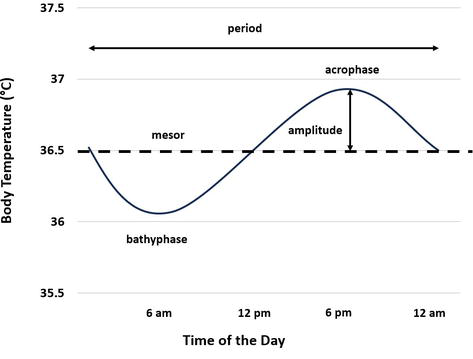
\includegraphics{SineSleep.png}
\end{center}

Text and figure from \textit{Human Body Temperature Circadian Rhythm in Health and Disease} by Written By Ivayla I. Geneva. \href{https://www.intechopen.com/chapters/89202}{DOI: 10.5772/intechopen.1003852}

Based on this passage, describe what to do with temperature measurements taken every 30 minutes while you are awake over the course of three days to find your ideal bedtime. \textbf{This is no substitute for actual medical advice; if you are having trouble with sleep, talk to a doctor!}

\fillwithlines{3in}

\end{questions}
\endgradingrange{all}
\clearpage

\bigskip

\begin{huge}Thank you\end{huge} for a wonderful semester, and please stay in touch if you are graduating! You can always find my up-to-date contact information at \href{https://crgibbons.github.io}{crgibbons.github.io} in case you would like to send a note or request a letter of recommendation or explain legalese to me when a new SCOTUS opinion drops.

If this course was fun but left you wishing for more ``how math makes us human'' discourse, you may wish to read \textit{Mathematics for Human Flourishing} by Francis Su. The book is an expanded version of a lecture delivered by Dr. Su in 2017, and I provide an excerpt from that lecture to conclude our semester together.

\begin{large}
\begin{quote}
The quest for truth is at the heart of the scientific enterprise.  I say `quest' because we don't do science to confirm simple declarative statements that are easily verified, like: ``my coffee is hot''.  Rather, our subject of investigation are questions for which the answer is not so clear.  ``Do gravity waves exist, and if so how would we detect them?''

So there is a quest.  We formulate a hypothesis (``they exist'') and we design experiments to test our hypotheses.  We look for evidence, and if we find some, we still ask: could there have been any other explanation?   

A mathematician might try to prove or disprove a statement through logical deductions from first principles. Or she might construct a mathematical model to answer the question. 

These approaches cultivate in us the virtue of \textbf{rigorous thinking}: the ability to handle ideas well, and craft clear arguments with those ideas.  This virtue serves us well in every area of life.  We should use this ability to reason in the public square, as many in our community have done by writing op-ed pieces for newspapers.

I would love to see more of us exercise this virtue, to shape public perceptions about mathematics. \hfill -Dr. Francis Su
\end{quote}
\end{large}
\vfill

\noindent Best wishes for whatever comes next for you, and I hope it includes lots of flourishing (with or without mathematics).
\end{document}
